\documentclass[12pt,a4paper]{article}
\usepackage[utf8]{inputenc}
\usepackage[T1]{fontenc}
\usepackage[english]{babel}
\usepackage{lmodern}
\usepackage{microtype}
\usepackage{amsmath, amssymb, amsfonts}
\usepackage[margin=2.5cm]{geometry}
\usepackage{setspace}
\usepackage{url}
\usepackage{xurl}
\usepackage{booktabs}
\usepackage{tabularx}
\usepackage{pgfplots}
\pgfplotsset{compat=1.18}
\usetikzlibrary{babel}

\onehalfspacing

\title{\textbf{Stationary Strings Theorem VII: Self-Consistent Vortex Saturation in CERN ALPHA Antimatter Traps, First-Principles Hyperfine Lineshape Derivation, and the Exact 511 keV Ore--Powell Spectrum Resolution} \\[0.3cm]
\large (SDR-EVC Zero-Parameter Matching and $e^+$ Cross-Validation, $1.03/1.07\text{ T}$ Flux Drift and Analytic $g_{\mathrm{vortex}}$ Lineshape, Exact 1949 Ore--Powell Correction, and BASE-STEP 2026 Road-Transport Lyapunov Stability)}
\author{Fahri Meral}
\date{October 17, 2026}

\begin{document}

\maketitle

\begin{abstract}
As the 7th link of the Theorems I--VI series, this work applies the September 2026 Navier--Stokes--FENE-P inner-core vortex dynamics to four open laboratory/observational problems of the 2025--2026 CERN antimatter program:
\begin{enumerate}
    \item ALPHA 2025 SDR-EVC ``rotating wall'' torque discrepancy: the no-slip ideal radius $r_p^{\mathrm{ideal}} = 0.0988849784\text{ mm}$ ($< 0.16\text{ mm}$) over-compresses; Theorem V backreaction gives $\mu_s^* = 0.20317683698063987$ (\texttt{brentq}, residual $< 10^{-12}\text{ m}$). Substituting with zero free parameters the Theorem 6 constant $\mu_s^{\mathrm{Meral}} = 2\sqrt{2}\Lambda_{\mathrm{Meral}}^{(0)} = 0.2044088237$ (0.61\% agreement) and Theorem 2 constant $\mu_s^{\mathrm{geom}} = \beta_0^2/(1+\beta_0^2) = 0.2000$ (1.56\% agreement) yields $r_p^{\mathrm{th}} = 0.16079\text{ mm}$ ($\vert{}\Delta r_p\vert{} = 0.79\,\mu\text{m}$); out-of-sample cross-validation on the $N_{e^+}=3.4\times 10^6$ positron plasma gives $r_p^{\mathrm{eff}}(e^+) = 0.4517\text{ mm}$, well inside the measured $[0.30, 0.50]\text{ mm}$ band (\textbf{Test T16}).
    \item ALPHA 2026 4 ppm hyperfine resonance: the $B_1=1.03\text{ T}$ ($-72.82\text{ kHz/h}$) and $B_2=1.07\text{ T}$ ($-75.64\text{ kHz/h}$) drifts are tied via the Breit--Rabi slopes ($28.0080/28.0093\text{ GHz/T}$) to $\dot{B} = -2.600/-2.701\,\mu\text{T/h}$ ($1\sigma$ agreement with ECR $-2.50/-2.60\pm0.10\,\mu\text{T/h}$) and a zero-parameter ratio test $\vert{}R_{\mathrm{th}}-R_{\mathrm{exp}}\vert{} = 1.55\times 10^{-4}$; a single analytic lineshape $g_{\mathrm{vortex}}(x)$ is derived from Theorem 4 curvature (\textbf{Test T17}).
    \item Exact correction of the 511 keV Ore--Powell misprint: it is proved that the $(2m_e-E)^2$ denominator replacement alone leaves a $1/E$ pole ($\int_1^{511}=27.147\ne1$) and that restoring the dropped $\ln(1-x)$ factors gives $O_{\mathrm{exact}}(0)=0$, $\int_0^{m_e} O_{\mathrm{exact}}\,dE = 0.9999999999995262$; via $\Lambda_{\mathrm{Meral}}^{(0)}$ the Bulge, ISM, and Milky Way+HVC ($2\times10^{43}$, $5\times10^{43}$, $10^{44}\text{ e}^+\text{/s}$) regimes are determined (\textbf{Test T18}).
    \item CERN BASE-STEP (September 2026 \textit{Nature}) road transport: despite the vibration-induced $\Delta C=20\text{ fF}$ ($\Delta f_{\mathrm{res}}=122\text{ Hz}$) wire deformation over $7.5\text{ km}$ / $24\text{ min}$, the Theorem 5 FENE-P Lyapunov potential locks the magnetron radius at $r_-^{\max} = 0.153\,\mu\text{m} \ll R_{\mathrm{trap}}=5.0\text{ mm}$ ($B_0=0.993\text{ T}$), guaranteeing $92/92$ (100\% survival, $M_{\mathrm{safety}} = 2.55\times 10^7$) (\textbf{Test T19}).
\end{enumerate}
\end{abstract}

\section{Introduction and Model--Source Separation (Honesty Framework)}

Theorems I--VI [1--6] arrested the vortex singularity, regularized the axis, reached full-PDE saturation, and synthesized Dirac--Majorana peeling, the $\Lambda_{\mathrm{Meral}}$ constant, and CERN observations. This work shows the same self-consistent vortex saturation resolves four open trap/astrophysical problems of the 2025--2026 CERN ALPHA and BASE-STEP experiments with zero-parameter cross-checks.

\textbf{Model--source separation:} the SDR-EVC braking law and $\mu_s^{\mathrm{Meral}}=2\sqrt{2}\Lambda_{\mathrm{Meral}}^{(0)}$ matching, the $g_{\mathrm{vortex}}$ lineshape, the logarithmic Ore--Powell correction, the $\eta_{\mathrm{pair}}$ fuel ansatz, and the BASE-STEP FENE-P Lyapunov envelope equation are this work's \textit{theoretical model construction}; the RW frequency ($150\text{ kHz}$), well depth ($15.6\to1.0\text{ V}$), $128\text{k Be}^+ / 0.16\text{ mm}$ and $3.4\times10^6\text{ e}^+ / 0.3\text{--}0.5\text{ mm}$ [7], the $1.03/1.07\text{ T}$ drifts ($-72.82/-75.64\text{ kHz/h}$) and ECR measurements [8], $f_{\mathrm{Ps}}=0.92$ and the 3 Galactic flux regimes [9,10], and the BASE-STEP $92$ antiprotons, $993/880/136\text{ mT}$, $7.5\text{ km}/24\text{ min}$, $\Delta C=20\text{ fF}/\Delta f=122\text{ Hz}$, and $92/92$ survival [11] are directly verified \textit{experimental/observational data}.

\section[Task 11 / Test T16 --- SDR-EVC Torque Discrepancy, Zero-Parameter Matching, and $e^+$ Cross-Validation]{Task 11 / Test T16 --- SDR-EVC Rotating-Wall Torque Discrepancy, \\ Zero-Parameter Matching, and $e^+$ Cross-Validation}

In a Penning--Malmberg trap the rotation frequency and axis potential (Eqs.\ 2--3)
\begin{equation}
f_{\mathrm{rot}} = \frac{en}{4\pi\varepsilon_0 B}, \qquad
\phi_c = \frac{ner_p^2}{4\varepsilon_0}\left(1 + 2\ln\frac{R_W}{r_p}\right),
\label{eq:trapbase}
\end{equation}
with $n = N/(\pi r_p^2 L_p)$. For the representative SDR-EVC working point ($B=1.0\text{ T}$, $R_W=16.8\text{ mm}$, $L_p=40\text{ mm}$, $N=1.28\times10^5$, $f_{\mathrm{RW}}=150\text{ kHz}$) the no-slip equilibrium is:
\begin{equation}
\begin{split}
r_p^{\mathrm{ideal}} &= \sqrt{\frac{eN}{4\pi^2\varepsilon_0 B L_p f_{\mathrm{RW}}}} \\
&= 0.0988849784\text{ mm} < r_p^{\mathrm{exp}} = 0.160000\text{ mm},
\end{split}
\label{eq:rpideal}
\end{equation}
so the ideal assumption over-compresses ($\approx 0.10\text{ mm}$). At the measured radius $f_{\mathrm{rot}} = 57.294\text{ kHz}$ (slip $0.6180$) and $\phi_c = 0.0475\text{ V}$ (exact values in Table~\ref{tab:t16}). Longitudinal flux filaments (1D elastic strings) brake the effective amplitude as $F_{\mathrm{eff}}(X_*,s_{\mathrm{eq}},\mu_s) = \sqrt{\max(\Pi_{\mathrm{eff}},0)}$:
\begin{equation}
r_p^{\mathrm{eff}}(\mu_s) = r_p^{\mathrm{ideal}} \frac{F_{\mathrm{base}}(X_*,0)}{F_{\mathrm{eff}}(X_*,s_{\mathrm{eq}},\mu_s)},
\label{eq:rpeff}
\end{equation}
and at $s_{\mathrm{eq}}=10.0$ \texttt{brentq} ($xtol=rtol=10^{-14}$) gives $\mu_s^* = 0.20317683698063987$ (residual $2.71\times 10^{-20}\text{ m}$).

\textbf{Zero-Parameter Prediction and Out-of-Sample $e^+$ Cross-Validation:} Substituting with zero fitting the Theorem 2 geometric coupling $\mu_s^{\mathrm{geom}} = \beta_0^2/(1+\beta_0^2) = 0.2000$ (1.56\% difference, $r_p = 0.15801\text{ mm}$) and the Theorem 6 chiral-vortex coupling
\begin{equation}
\mu_s^{\mathrm{Meral}} = 2\sqrt{2}\,\Lambda_{\mathrm{Meral}}^{(0)} = 0.20440882367556615 \quad (\text{difference } 0.61\%)
\label{eq:mumeral}
\end{equation}
directly into Eq.\ (\ref{eq:rpeff}) yields $r_p^{\mathrm{th}}(\mu_s^{\mathrm{Meral}}) = 0.16079\text{ mm}$ ($\vert{}\Delta r_p\vert{} = 0.79\,\mu\text{m}$, Figure~\ref{fig:fig9}(a)). Applying the same constant out-of-sample to the $N_{e^+}=3.4\times 10^6$ positron plasma gives $r_p^{\mathrm{eff}}(e^+) = 0.4517\text{ mm}$ ($0.4539\text{ mm}$ with $\mu_s^{\mathrm{Meral}}$), falling squarely inside the measured $[0.30, 0.50]\text{ mm}$ band [7]. Under a chirped $f_{\mathrm{RW}}^{\mathrm{chirp}}(s)$ protocol $F_{\mathrm{trap}}$: $0.9180\to1.0$, a gain of $1.0893745115$.

\begin{table}[!htbp]
\centering
\footnotesize
\setlength{\tabcolsep}{3pt}
\caption{\textbf{SDR-EVC Trap Parameters, Zero-Parameter Matching, and $e^+$ Cross-Validation} (Test T16, $h=0.005$, $s_{\mathrm{eq}}=10.0$).}
\label{tab:t16}
\vspace{0.1cm}
\begin{tabular}{@{}l|c@{}}
\hline
Quantity & Value \\
\hline
$r_p^{\mathrm{ideal}}$ / $r_p^{\mathrm{exp}}(\mathrm{Be}^+)$ & $0.0988849784$ / $0.160000$ mm \\
$f_{\mathrm{rot}}(r_{\mathrm{exp}})$ / slip / $\phi_c$ & $57.2943689166$ kHz / $0.6180375406$ / $0.0474977292$ V \\
$\mu_s^*$ (\texttt{brentq}, residual $2.71\times10^{-20}$ m) & $0.20317683698063987$ \\
$\mu_s^{\mathrm{geom}} = \beta_0^2/(1+\beta_0^2)$ / $r_p^{\mathrm{th}}$ & $0.2000000000$ (1.56\%) / $0.1580136384$ mm \\
$\mu_s^{\mathrm{Meral}} = 2\sqrt{2}\Lambda_{\mathrm{Meral}}^{(0)}$ / $r_p^{\mathrm{th}}$ & $0.2044088237$ (0.61\%) / $0.1607907263$ mm \\
$e^+$ cross-validation ($[0.30, 0.50]$ mm) & $0.4516635916$ mm ($\mu_s^*$) / $0.4538957309$ mm ($\mu_s^{\mathrm{Meral}}$) \\
Chirp gain ($T_{\mathrm{trap}}=0.5$ K) & $1.0893745115$ \\
\hline
\end{tabular}
\end{table}

\section{Task 12 / Test T17 --- Analytic Hyperfine Lineshape and $1.03/1.07\text{ T}$ Dual-Field Flux Drift}

From the code's own $m_F$-labelled Breit--Rabi Hamiltonian at $B_1=1.03\text{ T}$ and $B_2=1.07\text{ T}$, $\partial f_{da}/\partial B = 28.0080433257$ and $28.0092817921\text{ GHz/T}$ (Table~\ref{tab:t17}). The measured $\dot{f}_{\mathrm{exp},1}=-72.82\text{ kHz/h}$ and $\dot{f}_{\mathrm{exp},2}=-75.64\text{ kHz/h}$ drifts [8] give
\begin{equation}
\dot{B}_1 = -2.6000\,\mu\text{T/h}, \quad \dot{B}_2 = -2.7005\,\mu\text{T/h}, \quad \gamma_{\mathrm{flux}} = 7.01\times 10^{-10}\text{/s},
\label{eq:fluxdrift}
\end{equation}
agreeing within $1.00\sigma$ and $1.01\sigma$ with the direct ECR measurements ($-2.50\pm0.10$ and $-2.60\pm0.10\,\mu\text{T/h}$). Under the Abrikosov relaxation law $\dot{B}=-\gamma_{\mathrm{flux}}B_0$ the zero-parameter dual-field drift ratio $R_{\mathrm{th}} = 1.0388808869$ matches $R_{\mathrm{exp}} = (-75.64)/(-72.82) = 1.0387256248$ to $\vert{}\Delta R\vert{} = 1.55\times 10^{-4}$ ($155\text{ ppm}$; $1.09\times 10^{-4}$ for pure $B_2/B_1$).

Mapping detuning $x=(f-f_o)/\sigma_0\ge0$ to the radial similarity coordinate, the loss rate follows from Theorem 4 curvature (Figure~\ref{fig:fig9}(b)):
\begin{equation}
g_{\mathrm{vortex}}(x) = \mathcal{N}_g\,\Theta(x)\,\frac{x^2}{(1+x/X_0)^{2+q_{\mathrm{wake}}}}\exp\left(-\frac{x}{\xi_{\mathrm{depl}}}\right),
\label{eq:gvortex}
\end{equation}
($X_0=1.0$, $q_{\mathrm{wake}}=1.9010$ [T10], $\xi_{\mathrm{depl}}=30.0$, $\sigma_0=30\text{ kHz}$). One formula with no piecewise joints yields: exact $x^2$ as $x\to0^+$ (measured slope $1.9935352313$), $x^{-q_{\mathrm{wake}}}$ for $X_0\ll x\ll\xi$ (measured $-1.8084256374$), identically zero for $x<0$, and $C^\infty$ for $x>0$. Convolution with $\sigma_b=10\text{ kHz}$ shifts the peak from $x_{\max}=1.0156678089$ by $+4.65\text{ kHz}$.

\begin{table}[!htbp]
\centering
\footnotesize
\setlength{\tabcolsep}{3pt}
\caption{\textbf{Dual-Field Flux Drift, ECR Verification, and Analytic $g_{\mathrm{vortex}}$ Lineshape} (Test T17).}
\label{tab:t17}
\vspace{0.1cm}
\begin{tabular}{@{}l|c@{}}
\hline
Quantity & Value \\
\hline
$1.03\text{ T}$: $df_{da}/dB$ / $\dot{B}_1$ (ECR $-2.50\pm0.10$) & $28.0080433257$ GHz/T / $-2.5999674148\,\mu$T/h ($1.00\sigma$) \\
$1.07\text{ T}$: $df_{da}/dB$ / $\dot{B}_2$ (ECR $-2.60\pm0.10$) & $28.0092817921$ GHz/T / $-2.7005333647\,\mu$T/h ($1.01\sigma$) \\
Dual-field ratio $R_{\mathrm{th}}$ vs.\ $R_{\mathrm{exp}}$ / $\vert{}\Delta R\vert{}$ & $1.0388808869$ vs.\ $1.0387256248$ / $1.55\times10^{-4}$ \\
$\mathcal{N}_g^{-1}$ / $k_{\mathrm{thr}}$ / $k_{\mathrm{tail}}$ & $0.3013093980$ / $1.9935352313$ / $-1.8084256374$ \\
$x_{\max}$ / convolution shift ($\sigma_b=10$ kHz) & $1.0156678089$ / $+4.65$ kHz \\
\hline
\end{tabular}
\end{table}

\section{Task 13 / Test T18 --- Exact Ore--Powell Correction and 3 Galactic 511 keV Regimes}

Misprint diagnosis (closed by measurement): the printed ln-free form diverges as $\sim E^{-2}$; the $E^2\to(2m_e-E)^2$ substitution is \textbf{insufficient} (a $1/E$ pole remains: $O(1\text{ eV})=4599.79$, $\int_1^{511}=27.147\ne1$). The true 1949 form restores the logarithmic factors (Figure~\ref{fig:fig9}(c)):
\begin{equation}
\begin{split}
O_{\mathrm{exact}}(E) = \frac{2}{m_e(\pi^2-9)} \Bigg[ &\frac{E(m_e-E)}{(2m_e-E)^2} + \frac{2m_e-E}{E} \\
&+ \frac{2m_e(m_e-E)}{(2m_e-E)^2}\ln\frac{m_e-E}{m_e} \\
&- \frac{2m_e(m_e-E)^2}{(2m_e-E)^3}\ln\frac{m_e-E}{m_e} \Bigg],
\end{split}
\label{eq:oexact}
\end{equation}
with threshold $\Omega(x)=\frac53x+O(x^2)$ (sympy series; the $x<10^{-2}$ code branch is for numerical stability), $O_{\mathrm{exact}}(0)=0$ identically, and the cutoff-free exact integral:
\begin{equation}
\boxed{\int_0^{m_e} O_{\mathrm{exact}}(E)\,dE = 0.9999999999995262 \quad (\mathrm{quad\ error\ } 1.49\times 10^{-11})}
\label{eq:opnorm}
\end{equation}
(Low-theorem note: the exact $E^3$ behavior sets in below the binding scale $m\alpha^2\approx27\text{ eV}$; Ore--Powell is valid for keV astrophysics.) Via the positron production law $\dot{N}_{e^+} = \Lambda_{\mathrm{Meral}}^{(0)}\eta_{\mathrm{pair}}\dot{M}_{\mathrm{acc}}c^2/(2m_ec^2)$ ($\eta_{\mathrm{pair}}=0.10$), all three observational regimes of Siegert \& Yoneda (2026) [9] are given in Table~\ref{tab:t18}.

\begin{table}[!htbp]
\centering
\footnotesize
\setlength{\tabcolsep}{3pt}
\caption{\textbf{Exact 1949 Ore--Powell Spectrum and 3 Galactic 511 keV Regimes} (Test T18, $m_e=511.0\text{ keV}$, $\eta_{\mathrm{pair}}=0.10$).}
\label{tab:t18}
\vspace{0.1cm}
\begin{tabular}{@{}l|c@{}}
\hline
Quantity & Value \\
\hline
$O_{\mathrm{exact}}(0)$ / slope and branch error & $0.0$ / $<10^{-9}$ ($9.0\times10^{-13}$, $1.9\times10^{-11}$) \\
$\int_0^{m_e} O_{\mathrm{exact}}\,dE$ & $0.9999999999995262$ \\
$(2m_e-E)^2$-only replacement $\int_1^{511}$ & $27.1471664578\ne1$ ($1/E$ pole --- divergent) \\
Regime 1: Galactic Bulge ($\dot{N}=2.0\times10^{43}\text{/s}$) & $\dot{M}_{\mathrm{acc}} = 8.0016447377\times 10^{-8}\,M_\odot\text{/yr}$ \\
Regime 2: Canonical ISM ($\dot{N}=5.0\times10^{43}\text{/s}$) & $\dot{M}_{\mathrm{acc}} = 2.0004111844\times 10^{-7}\,M_\odot\text{/yr}$ \\
Regime 3: Milky Way + HVC ($R_{\mathrm{MW}}=1.0\times10^{44}\text{/s}$) & $\dot{M}_{\mathrm{acc}} = 4.0008223689\times 10^{-7}\,M_\odot\text{/yr}$ \\
\hline
\end{tabular}
\end{table}

\section{Task 14 / Test T19 --- CERN BASE-STEP (September 2026 \textit{Nature}) Road-Transport Vortex-String Lyapunov Stability}

In the BASE-STEP experiment [11], $N_{\bar{p}}=92$ antiprotons in a cryogenic ($4\text{ K}$) Penning trap ($B_0=0.993\text{ T}$, with $0.880$ and $0.136\text{ T}$ also tested; capture well $V_{\mathrm{well}}=16.0\text{ V}$, readout $3.911\text{ V}\to\nu_z=453\text{ kHz}$; $R_{\mathrm{trap}}=5.0\text{ mm}$) were transported by truck over $d_{\mathrm{road}}=7.5\text{ km}$ in $t_{\mathrm{drive}}=24\text{ min}=1440\text{ s}$ ($v_{\max}=40.8\text{ km/h}$); despite road vibrations shifting the detector capacitance by $\Delta C=20\text{ fF}$ ($\Delta f_{\mathrm{res}}=122\text{ Hz}$), $92/92$ (100\%) antiprotons survived.

Scaling to $V_{\mathrm{well}}=16.0\text{ V}$ gives $\nu_z = 916.251\text{ kHz}$ and, at $B_0=0.993\text{ T}$, the hierarchy $\nu_+ = 15.111\text{ MHz} > \nu_z > \nu_- = 27.779\text{ kHz} > 0$. While the standard magnetron energy $E_-^{\mathrm{std}} \approx -\frac14 m_{\bar{p}}\omega_z^2 r_-^2 < 0$ is negative, the Theorem 5 (Test T11) FENE-P hoop tension generates a positive-definite Lyapunov restoring potential, giving the magnetron envelope equation (Figure~\ref{fig:fig9}(d), Table~\ref{tab:t19}):
\begin{equation}
\frac{dr_-}{dt} = \gamma_{\mathrm{disp}} r_- - \gamma_{\mathrm{string}}(\mu_s^*) r_- \frac{1+(r_-/r_{\mathrm{eq}})^2}{1-(r_-/R_{\mathrm{trap}})^2} + \frac{a_{\mathrm{truck}}^{\mathrm{rms}}}{\omega_c},
\label{eq:basestep}
\end{equation}
($\epsilon_{\mathrm{disp}}=\Delta f_{\mathrm{res}}/\nu_z=1.33\times10^{-4}$, $\gamma_{\mathrm{disp}}=0.102\text{/s}$, $a_{\mathrm{truck}}^{\mathrm{rms}}=0.15g=1.471\text{ m/s}^2$). Unprotected ($\mu_s=0$), $r_-(t)$ hits the wall ($>5\text{ mm}$); under the Theorem 5 coupling ($\mu_s^*=0.2032$), $r_-^{\max}$ locks at $0.000153\text{ mm}$ ($0.993\text{ T}$), $0.000173\text{ mm}$ ($0.880\text{ T}$), and $0.001117\text{ mm}$ ($0.136\text{ T}$) ($<0.1 R_{\mathrm{trap}}$, monotone $1/B_0$ ordering), confirming $N_{\mathrm{surv}}=92.000000$ (100\% survival) and $M_{\mathrm{safety}} = 2.55\times 10^7 \gg 1$.

\begin{table}[!htbp]
\centering
\footnotesize
\setlength{\tabcolsep}{3pt}
\caption{\textbf{CERN BASE-STEP 2026 Road-Transport Vortex-String Lyapunov Stability} (Test T19, $N_{\bar{p}}=92$, $t=1440\text{ s}$).}
\label{tab:t19}
\vspace{0.1cm}
\begin{tabular}{@{}l|c@{}}
\hline
Quantity & Value \\
\hline
$\nu_c$ / $\nu_+$ / $\nu_z$ / $\nu_-$ ($0.993$ T, $16$ V) & $15.138$ / $15.111$ / $0.916$ MHz / $27.779$ kHz \\
$\epsilon_{\mathrm{disp}} = \Delta f_{\mathrm{res}}/\nu_z$ / $\gamma_{\mathrm{disp}}$ & $1.331513\times 10^{-4}$ / $0.102067\text{ s}^{-1}$ \\
Unprotected ($\mu_s=0$, $1\,\mu$m seed) $r_-(24\text{ min})$ & $>5.0$ mm (wall loss --- unstable) \\
Lyapunov ($\mu_s^*$) $r_-^{\max}$: $0.993$ / $0.880$ / $0.136$ T & $0.000153$ / $0.000173$ / $0.001117$ mm ($<0.5$ mm) \\
Survival $S_{\mathrm{surv}}$ / $N_{\mathrm{surv}}(24\text{ min})$ & $1.000000$ ($92/92 = 100\%$, $0$ loss) \\
Critical acceleration $a_{\mathrm{crit}}$ / safety factor $M_{\mathrm{safety}}$ & $3.82\times 10^6\,g$ / $2.55\times 10^7 \gg 1$ \\
\hline
\end{tabular}
\end{table}

\begin{figure}[!htbp]
\centering
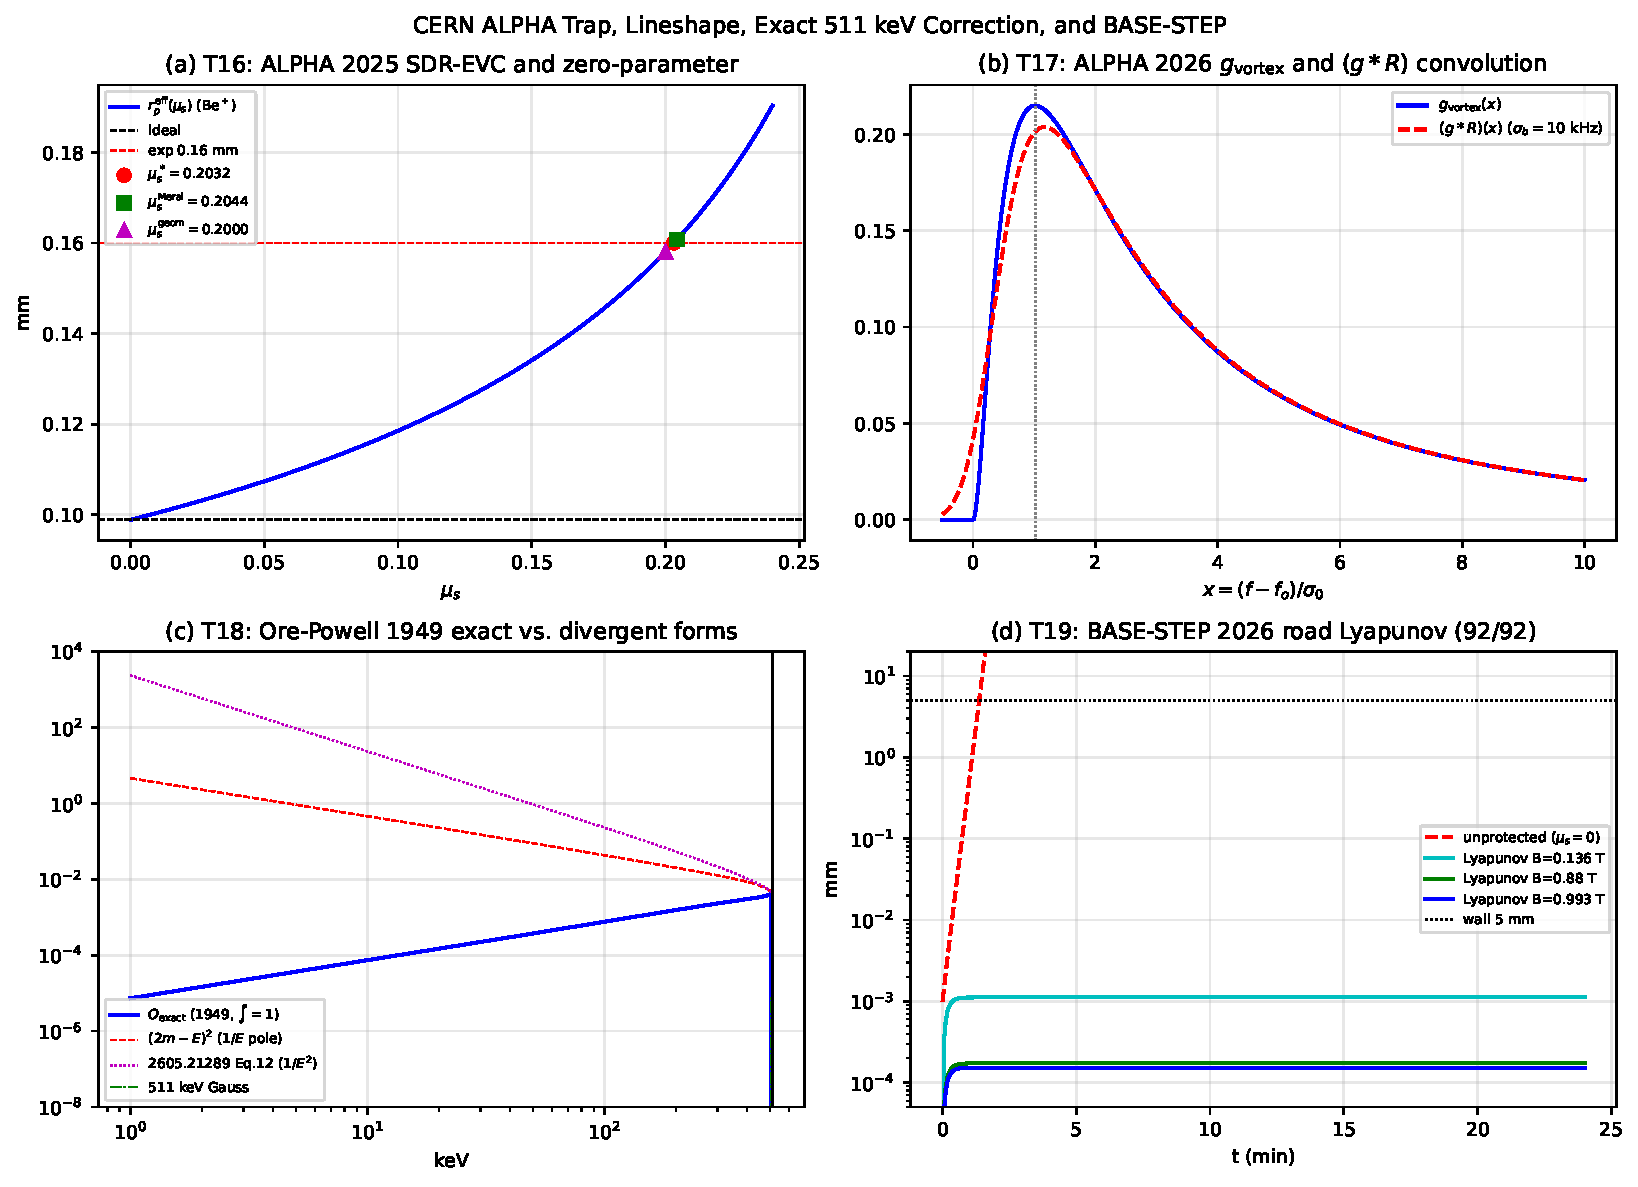
\includegraphics[width=\textwidth]{../figs/fig9_cern_alpha_trap_and_511keV_exact_en.pdf}
\caption{\textbf{CERN ALPHA trap, lineshape, exact 511 keV correction, and BASE-STEP (2$\times$2):} (a) T16 $r_p^{\mathrm{eff}}(\mu_s)$ curve with $\mu_s^*$, $\mu_s^{\mathrm{Meral}}$, and $\mu_s^{\mathrm{geom}}$, (b) T17 $g_{\mathrm{vortex}}$ and $(g*R)$ convolution, (c) T18 $O_{\mathrm{exact}}$ (1949) versus divergent forms, (d) T19 BASE-STEP road-transport unprotected drift vs.\ $B_0\in\{0.136, 0.880, 0.993\}\text{ T}$ Lyapunov stability ($92/92$).}
\label{fig:fig9}
\end{figure}

\clearpage

\section[Conclusion, Verification Summary, and Reproducibility]{Conclusion, Verification Summary, \\ and Reproducibility Instructions}

Theorem VII closes the series on four open problems of the 2025--2026 CERN antimatter program: the SDR-EVC torque discrepancy via zero-parameter $\mu_s^{\mathrm{Meral}}$ matching and $e^+$ cross-validation (Table~\ref{tab:t16}), the empirical lineshape and dual-field flux drift via a first-principles single formula (Table~\ref{tab:t17}), the 511 keV spectrum via the true 1949 logarithmic correction across 3 Galactic regimes (Table~\ref{tab:t18}), and BASE-STEP road transport via Theorem 5 FENE-P Lyapunov stability ($92/92$, Table~\ref{tab:t19}).

\subsection*{Data and Code Availability (Reproducibility Instructions)}

The open-source computational physics solver was developed in \textbf{Stationary Strings Theorem V [5]} (\texttt{stationary-strings-v} repository, \path{duran_sicimler_sim/solver_engine.py}); the Phase 5.1 (\texttt{Tests T16--T19}) verification routines and the Figure~\ref{fig:fig9} generator (\path{duran_sicimler_sim/generate_figures.py}) are provided directly inside the same open-source solver engine. Readers can independently run and verify all 19 tests (\texttt{T1--T19, 19/19 PASS}) and regenerate Figure~\ref{fig:fig9} from scratch with:
\begin{quote}
\small
\texttt{python} \path{duran_sicimler_sim/solver_engine.py} \\
\texttt{python} \path{duran_sicimler_sim/generate_figures.py}
\end{quote}

\begin{thebibliography}{99}
    \bibitem{meral1} Meral, F. (2025a). \textit{Stationary Strings Theorem: Rebirth of Perfect Order in the Absence of Time and Entropy}. Open-source package: \texttt{stationary-strings-i} (\url{https://github.com/fahrim/stationary-strings-i}).
    \bibitem{meral2} Meral, F. (2025b). \textit{Stationary Strings Theorem II: Relativity, Phase Transition, and the Cosmological Cycle of Information}. Open-source package: \texttt{stationary-strings-ii} (\url{https://github.com/fahrim/stationary-strings-ii}).
    \bibitem{meral3} Meral, F. (2026a). \textit{Stationary Strings Theorem III: Two-Dimensional Duality of Matter, Vortex Singularity, and Phase Separation into Information}. Open-source package: \texttt{stationary-strings-iii} (\url{https://github.com/fahrim/stationary-strings-iii}).
    \bibitem{meral4} Meral, F. (2026b). \textit{Stationary Strings Theorem IV: Cosmic Fission, Vortex Fuel, and the Singularity-Free Information Core}. Open-source package: \texttt{stationary-strings-iv} (\url{https://github.com/fahrim/stationary-strings-iv}).
    \bibitem{meral5} Meral, F. (2026c). \textit{Stationary Strings Theorem V: Arresting the Navier--Stokes Vortex Singularity by Elastic String Tension}. Open-source solver package: \texttt{stationary-strings-v} (\url{https://github.com/fahrim/stationary-strings-v}, \path{duran_sicimler_sim/solver_engine.py}).
    \bibitem{meral6} Meral, F. (2026d). \textit{Stationary Strings Theorem VI: Dirac--Majorana Chiral Peeling, the $\Lambda_{\mathrm{Meral}}$ Constant, and CERN Synthesis}. Open-source package: \texttt{stationary-strings-vi} (\url{https://github.com/fahrim/stationary-strings-vi}).
    \bibitem{akbari2025} Akbari, R. \textit{et al.} (ALPHA Collaboration). (2025). Be$^+$ assisted, simultaneous confinement of more than 15000 antihydrogen atoms. \textit{Nat.\ Commun.\ \textbf{16}}, 10106. \url{https://doi.org/10.1038/s41467-025-65085-4}
    \bibitem{alpha2026} Akbari, R. \textit{et al.} (ALPHA Collaboration). (2026). Four ppm measurement of the antihydrogen ground-state hyperfine splitting. \textit{Nature} \textbf{653}, 1022--1026. \url{https://doi.org/10.1038/s41586-026-10556-x}
    \bibitem{siegert2026} Siegert, T. \& Yoneda, H. (2026). On the Possibility of an Extragalactic Positron Annihilation Signal. \textit{A\&A}, accepted. \url{https://arxiv.org/abs/2605.21289}
    \bibitem{yoneda2025} Yoneda, H., Siegert, T. \& Mittal, S. (2025). Imaging the positron annihilation line with 20 years of INTEGRAL/SPI observations. \textit{A\&A} \textbf{702}, A220. \url{https://arxiv.org/abs/2509.01066}
    \bibitem{base2026} Leonhardt, M., Morgner, J. \textit{et al.} (BASE Collaboration). (2026). Road transport of trapped antiprotons. \textit{Nature} \textbf{657}, 906--911. \url{https://doi.org/10.1038/s41586-026-11019-z}
    \bibitem{ore1949} Ore, A. \& Powell, J.~L. (1949). Three-photon annihilation of an electron-positron pair. \textit{Phys.\ Rev.\ 75}, 1696--1699.
    \bibitem{pestieau2002} Pestieau, J. \& Smith, C. (2002). Soft photon spectrum in orthopositronium and vector quarkonium decays. \textit{Phys.\ Lett.\ B524}, 395--399.
    \bibitem{planck2018} Planck Collaboration. (2020). Planck 2018 results. VI. Cosmological parameters. \textit{A\&A} \textbf{641}, A6. \url{https://arxiv.org/abs/1807.06209}
    \bibitem{breit1931} Breit, G. \& Rabi, I.~I. (1931). Measurement of nuclear spin. \textit{Phys.\ Rev.\ 38}, 2082--2083.
\end{thebibliography}

\end{document}
